\begin{figure}[!h]
\begin{center}
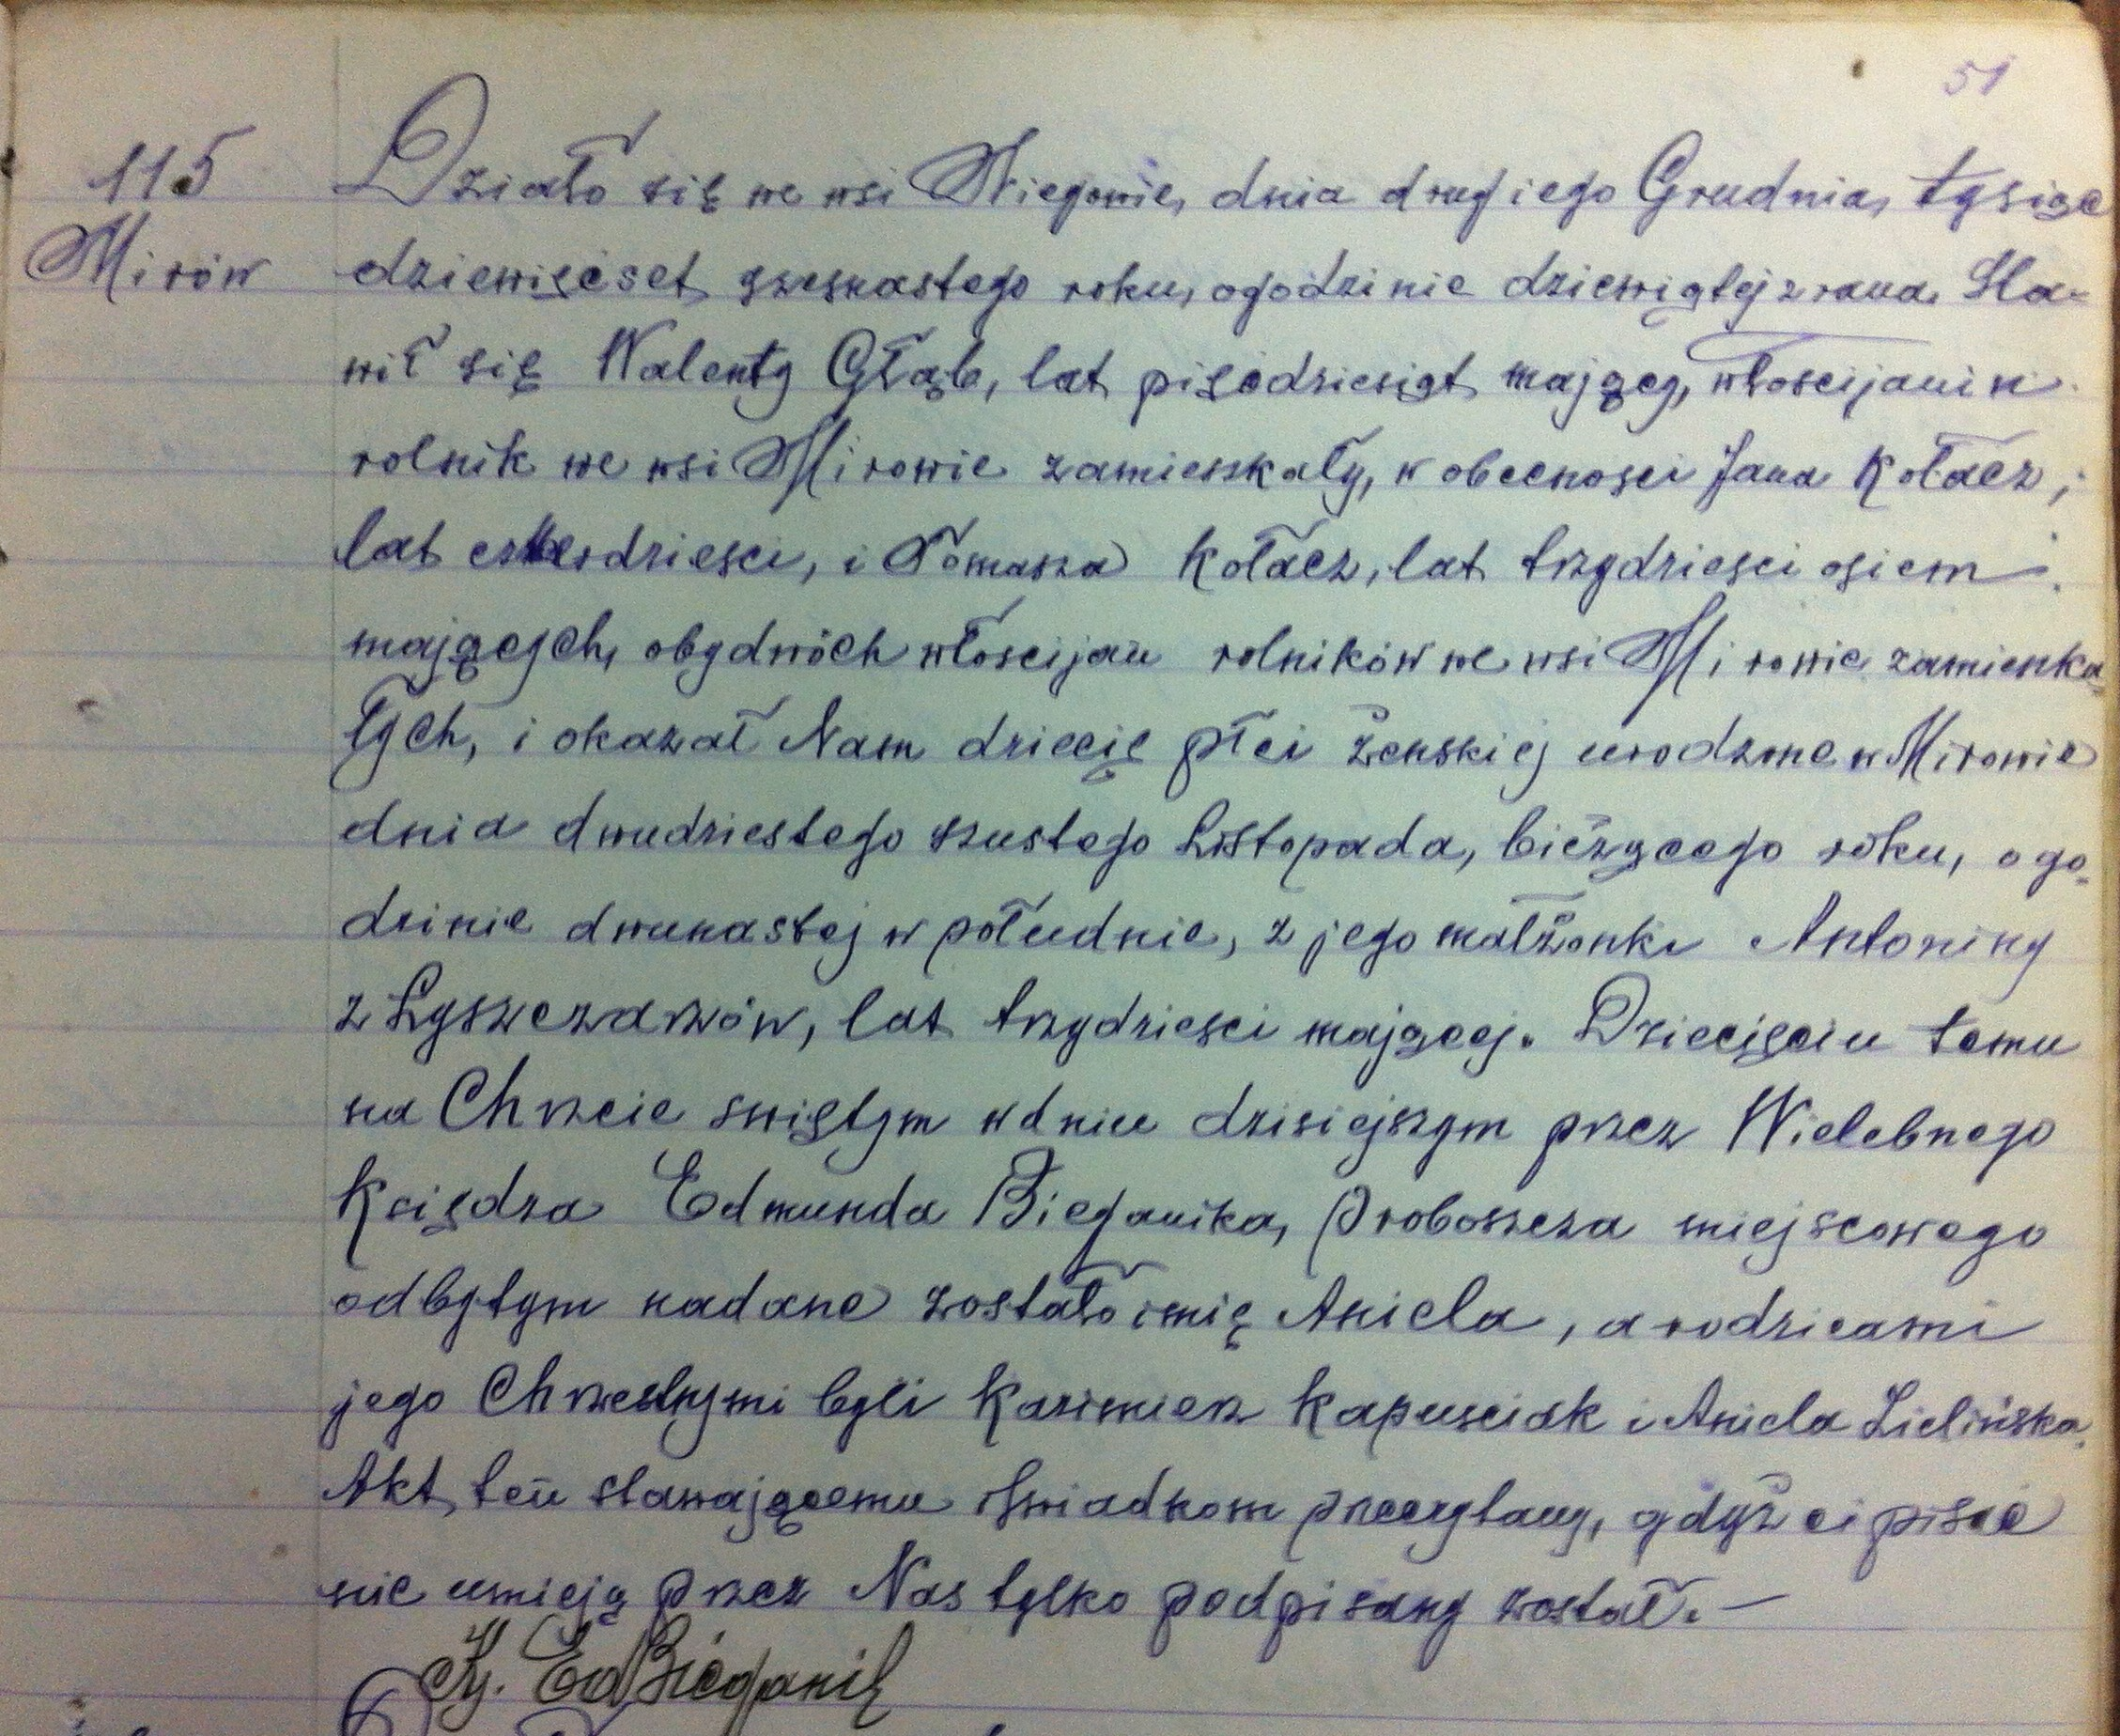
\includegraphics[width=0.8\textwidth]{zdjecia/akt_urodzenia_anieli_glab.jpg}
\caption{Akt urodzenia Anieli Głąb}
\label{rys:akt_urodzenia_anieli_glab}
\end{center}
\end{figure}

Aniela Głąbówna, najmłodsza córka Walentego i Antoniny Głąbów urodziła się 26 XI 1916 r. w Mirowie.

Wyszła ona za Karola Biskupskiego (ur. 5 V 1918 r. w Hanowerze), z którym przeżyła ponad 50 lat nie doczekawszy się własnego potomstwa. W związku z tym wzięli na wychowanie Barbarę (już wcześniej wymienioną) córkę Franciszka -- brata Anieli. Jako przybrani rodzice wypełniali przykładnie swe wobec niej obowiązki taty i mamy. Wybudowali nowy dom na poniemieckiej posesji i opiekowali się troskliwie swymi ,,przyszywanymi'' wnukami. Karol Biskupski zmarł 28 grudnia 2005 r. w Ligocie Dolnej. Aniela zaś zmarła w Kluczborku 30 stycznia 2010 r. Karol w czasie wojny przebywał w obozie koncentracyjnym w Auschwitz.

\begin{figure}[!h]
\begin{center}
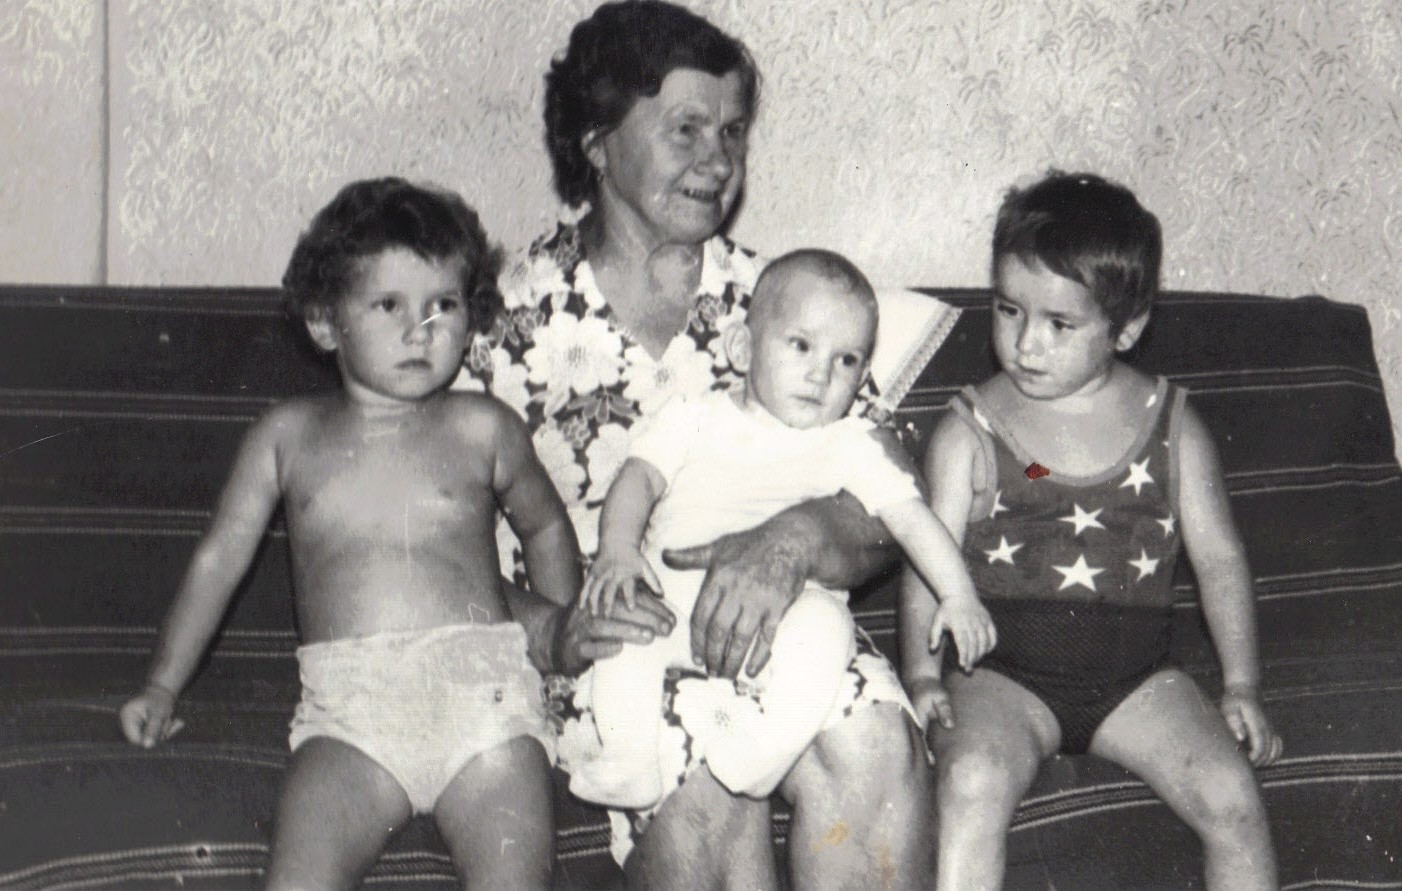
\includegraphics[width=0.7\textwidth]{zdjecia/aniela_biskupska_z_wnuczkami.jpg}
\caption[Aniela Biskupska z wnuczkami]{Aniela Biskupska z ,,wnuczkami'', od lewej: Kasia, Irek (na kolanach babci) i~Krzysiek Wilkowie}
\label{rys:aniela_biskupska_z_wnuczkami}
\end{center}
\end{figure}


% który zataił fakt, że w tym czasie był żonaty z inną kobietą na Ukrainie, gdzie mieszkał do czasu, gdy znalazł się w KL Auschwitz. Tamtejszy Kościół nadesłał jednak po kilku latach do Kurii Wrocławskiej informację o tym fakcie, co unieważniało automatycznie małżeństwo Anieli Głąbówny. Nie wiadomo, czy Karol Biskupski interesował się losem swej dotychczasowej, prawowitej małżonki oraz jak długo żyła. Może przeżyła swego prawowitego męża? Może ów Karol znał miejsce zamieszkania swej dotychczasowej małżonki i liczył na to, że zejdzie z tego świata przed nim i przed Anielą, co umożliwiłoby z nią prawowity ślub kościelny. Bo czymże wytłumaczyć fakt niedopełnienia przez niego przynajmniej formalności ślubu cywilnego. W tej sytuacji Aniela Głąbówna przeżywszy z Karolem Biskupskim ponad 50 lat nie otrzymała po nim żadnych praw współmałżonka! 
